%%%%%%%%%%%%%%%%%%%%%%%%%%%%%%%%%%%%%%%%%%%%%%%%%%%%%%%%%%%%%%%
%
% Welcome to Overleaf --- just edit your LaTeX on the left,
% and we'll compile it for you on the right. If you open the
% 'Share' menu, you can invite other users to edit at the same
% time. See www.overleaf.com/learn for more info. Enjoy!
%
%%%%%%%%%%%%%%%%%%%%%%%%%%%%%%%%%%%%%%%%%%%%%%%%%%%%%%%%%%%%%%%


% Inbuilt themes in beamer
\documentclass{beamer}

% Theme choice:
\usetheme{CambridgeUS}

 \providecommand{\pr}[1]{\ensuremath{\Pr\left(#1\right)}}
 \providecommand{\sbrak}[1]{\ensuremath{{}\left[#1\right]}}
 \providecommand{\brak}[1]{\ensuremath{\left(#1\right)}}
 \providecommand{\cbrak}[1]{\ensuremath{\left\{#1\right\}}}
% Title page details: 
\title{Assignment 7} 
\author{Donal Loitam - AI21BTECH11009}
\date{\today}
\logo{\large \LaTeX{}}

\usepackage{hyperref}
\usepackage{mathtools}
\usepackage{amssymb}
\usepackage{amsmath}


\begin{document}

% Title page frame
\begin{frame}
    \titlepage 
\end{frame}

% Remove logo from the next slides
\logo{}


% Outline frame
\begin{frame}{Papoulis ch2 problem 2.2}
TABLE OF CONTENTS
    \tableofcontents
\end{frame}


% Lists frame
\section{Question}
\begin{frame}{Problem}
If $A = \cbrak{2 \le x \le 5}$ and $B = \cbrak{3 \le x \le 6}$, find :
\begin{enumerate}
\item A + B 
\item AB and 
\item \brak{A + B}\brak{AB}'
\end{enumerate}
\end{frame}
% Q)Show that 
% \begin{itemize}
%     \item  (a) If $Pr(A) = Pr(B) = Pr(AB)$, then $Pr(A\bar{B} + B\bar{A})$ = 0
%     \item  (b) If $Pr(A) = Pr(B) = 1$, then $Pr(AB)$ = 1
% \end{itemize}


\section{Solution}
\begin{frame}{Solution}
    If $A = \cbrak{2 \le x \le 5}$ , $B = \cbrak{3 \le x \le 6}$ , $S = \cbrak{-\infty < x < \infty }$ then \\\\
    \begin{enumerate}
            \item $ A + B = \cbrak{2 \le x \le 6} $
            \item $ AB = \cbrak{3 \le x \le 5} $ \label{1} 
            \item  From  \eqref{1} and \\
            $\begin{aligned}[t]
           \because \brak{AB}'  &= S - \brak{AB} \\ 
              \implies  \brak{AB}' &= \cbrak{-\infty < x < \infty } - \cbrak{3 \le x \le 5} \\
             \implies \brak{AB}' &= \cbrak {\cbrak{x < 3} + \cbrak{x > 5} } \\\\
             \end{aligned} $
             \begin{align}
             Now , \brak{A + B}\brak{AB}' &= \cbrak{2 \le x \le 6} \cbrak {\cbrak{x < 3} + \cbrak{x > 5} } \\
                                          &= \cbrak{2 \le x < 3} + \cbrak{5 < x \le 6}
             \end{align} 
    \end{enumerate}
\end{frame}

\section{Verify from graph}
\begin{frame}{Graph}
The graphs  plotted via matplotlib verifies the solution :-\\
Here , $A = \cbrak{2 \le x \le 5} = blue $ and $B = \cbrak{3 \le x \le 6} = green$
\begin{figure}[!ht]
		\centering
		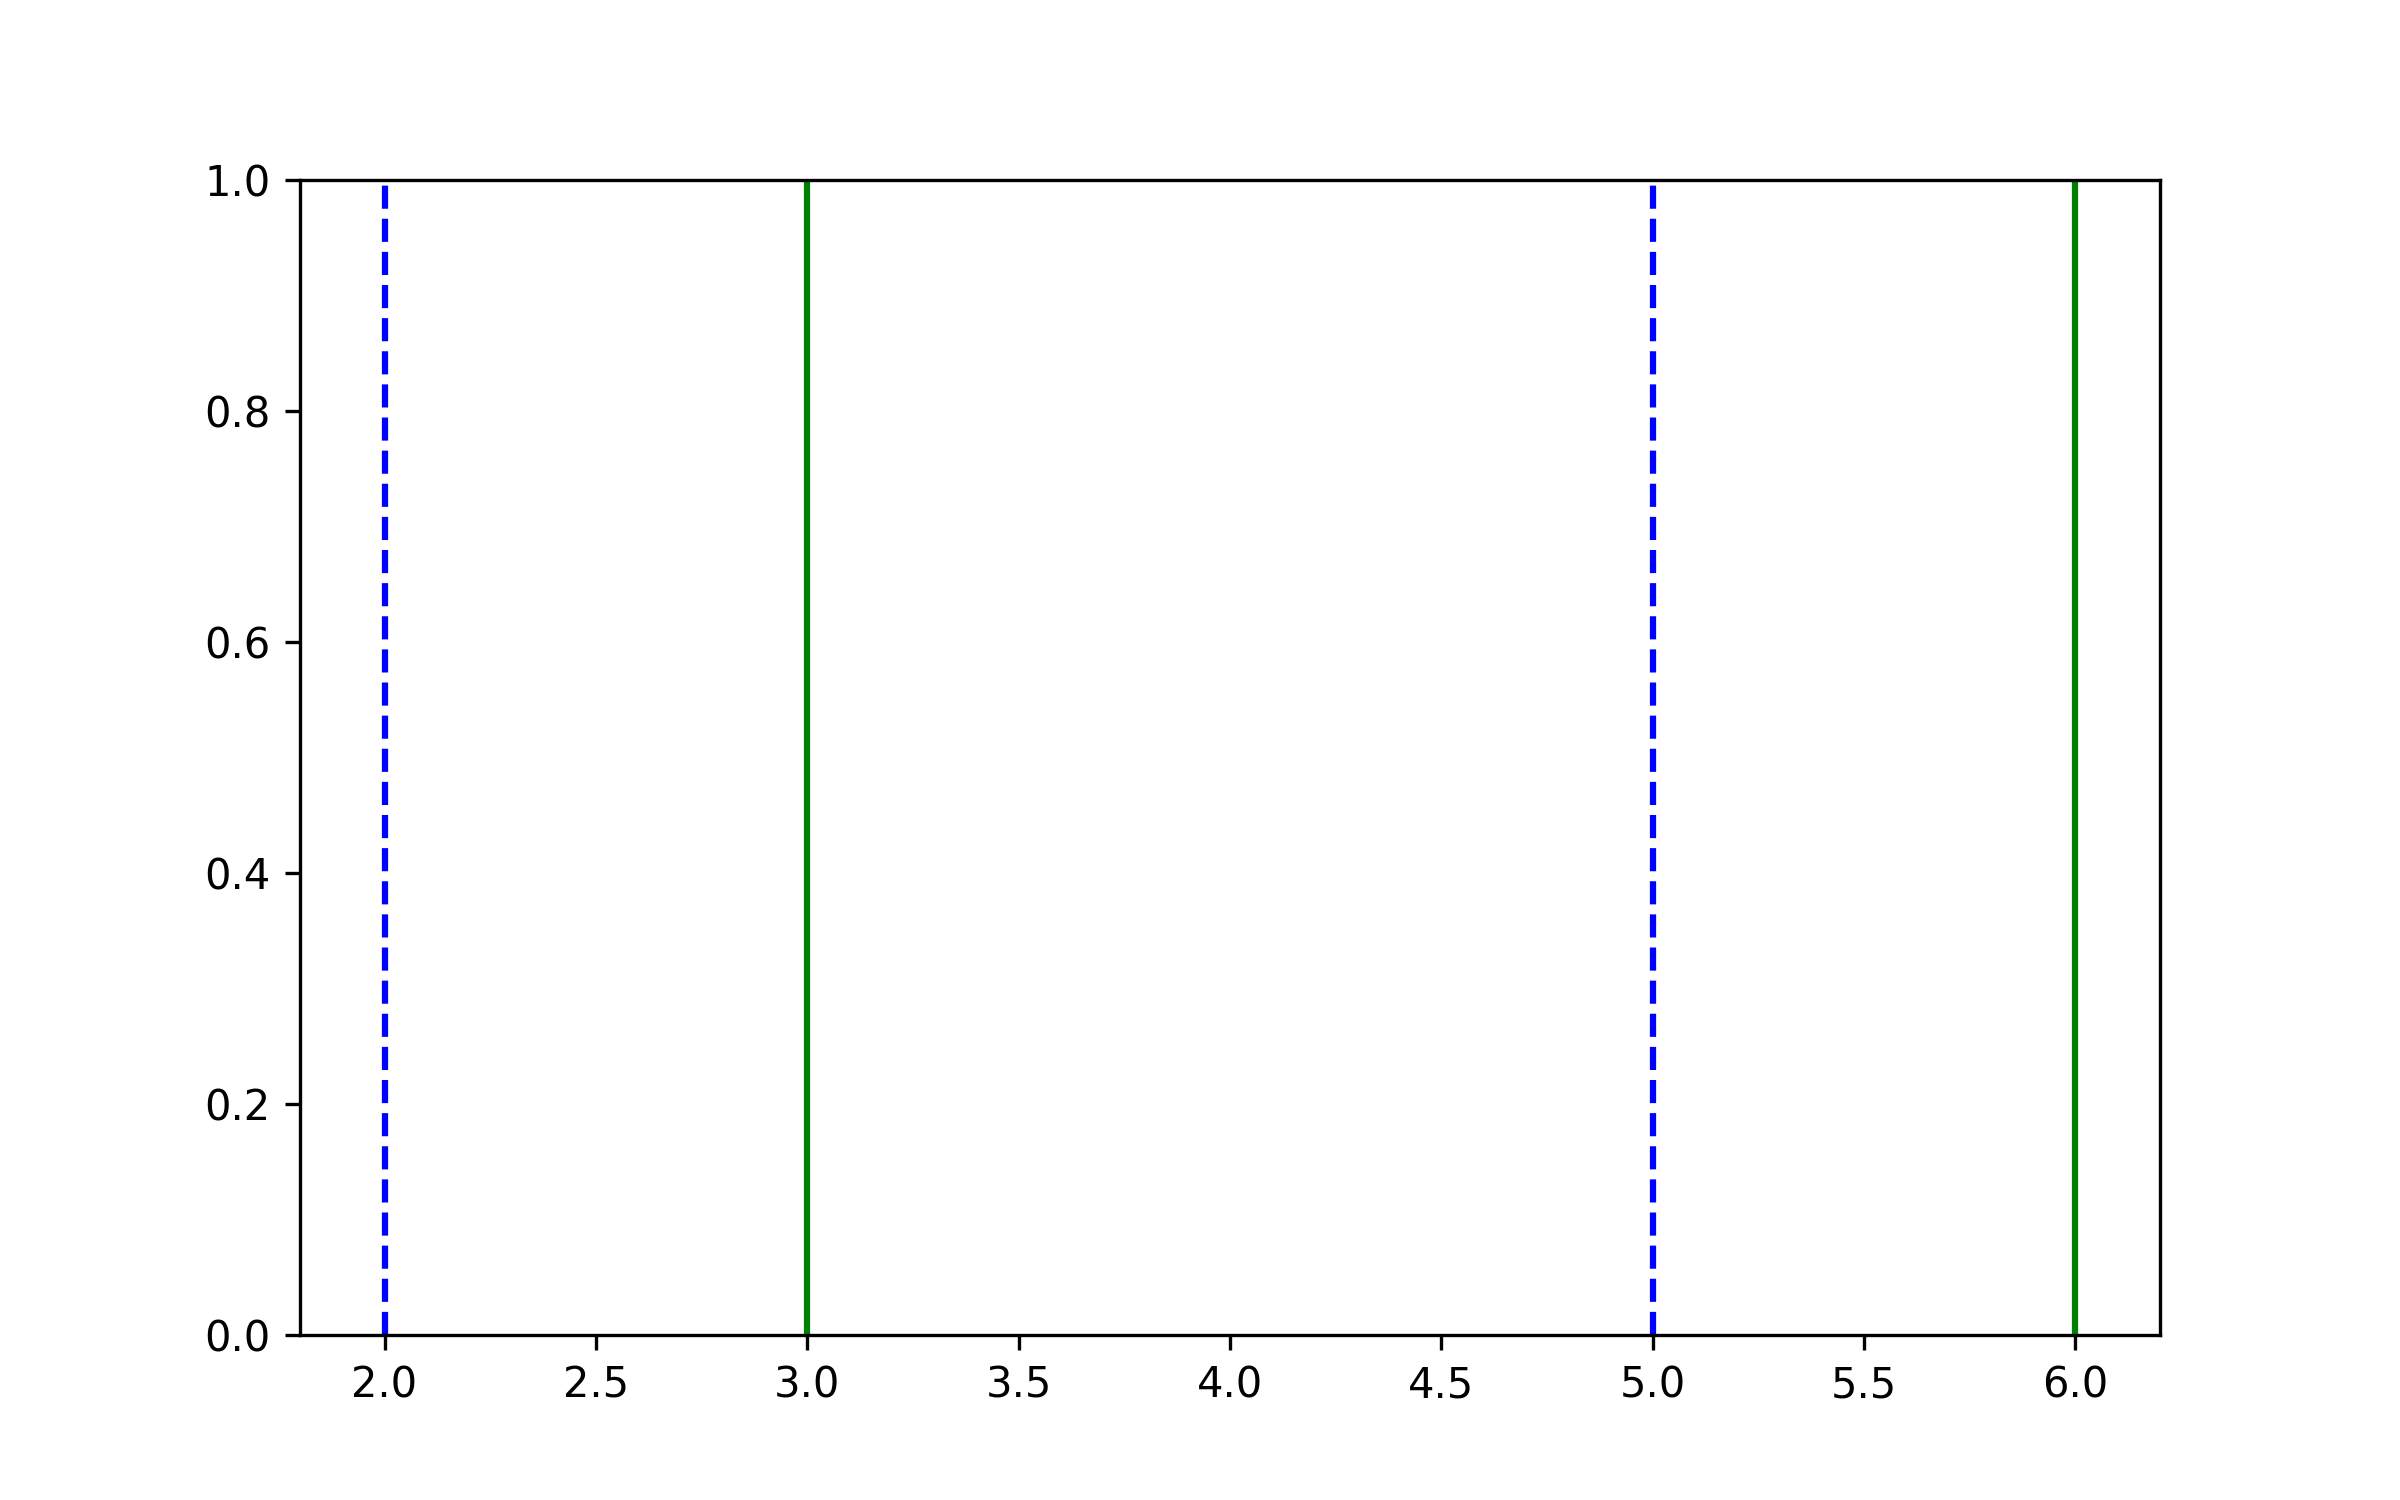
\includegraphics[width=0.75\textwidth]{line.png}
		\caption{Graph of A and B }
		\label{fig-1}
	\end{figure}
\end{frame}

\begin{frame}{Graph}
 \brak{A + B} = \brak{blue + dark green + green} , AB =  dark green 
   \begin{figure}[!ht]
		\centering
		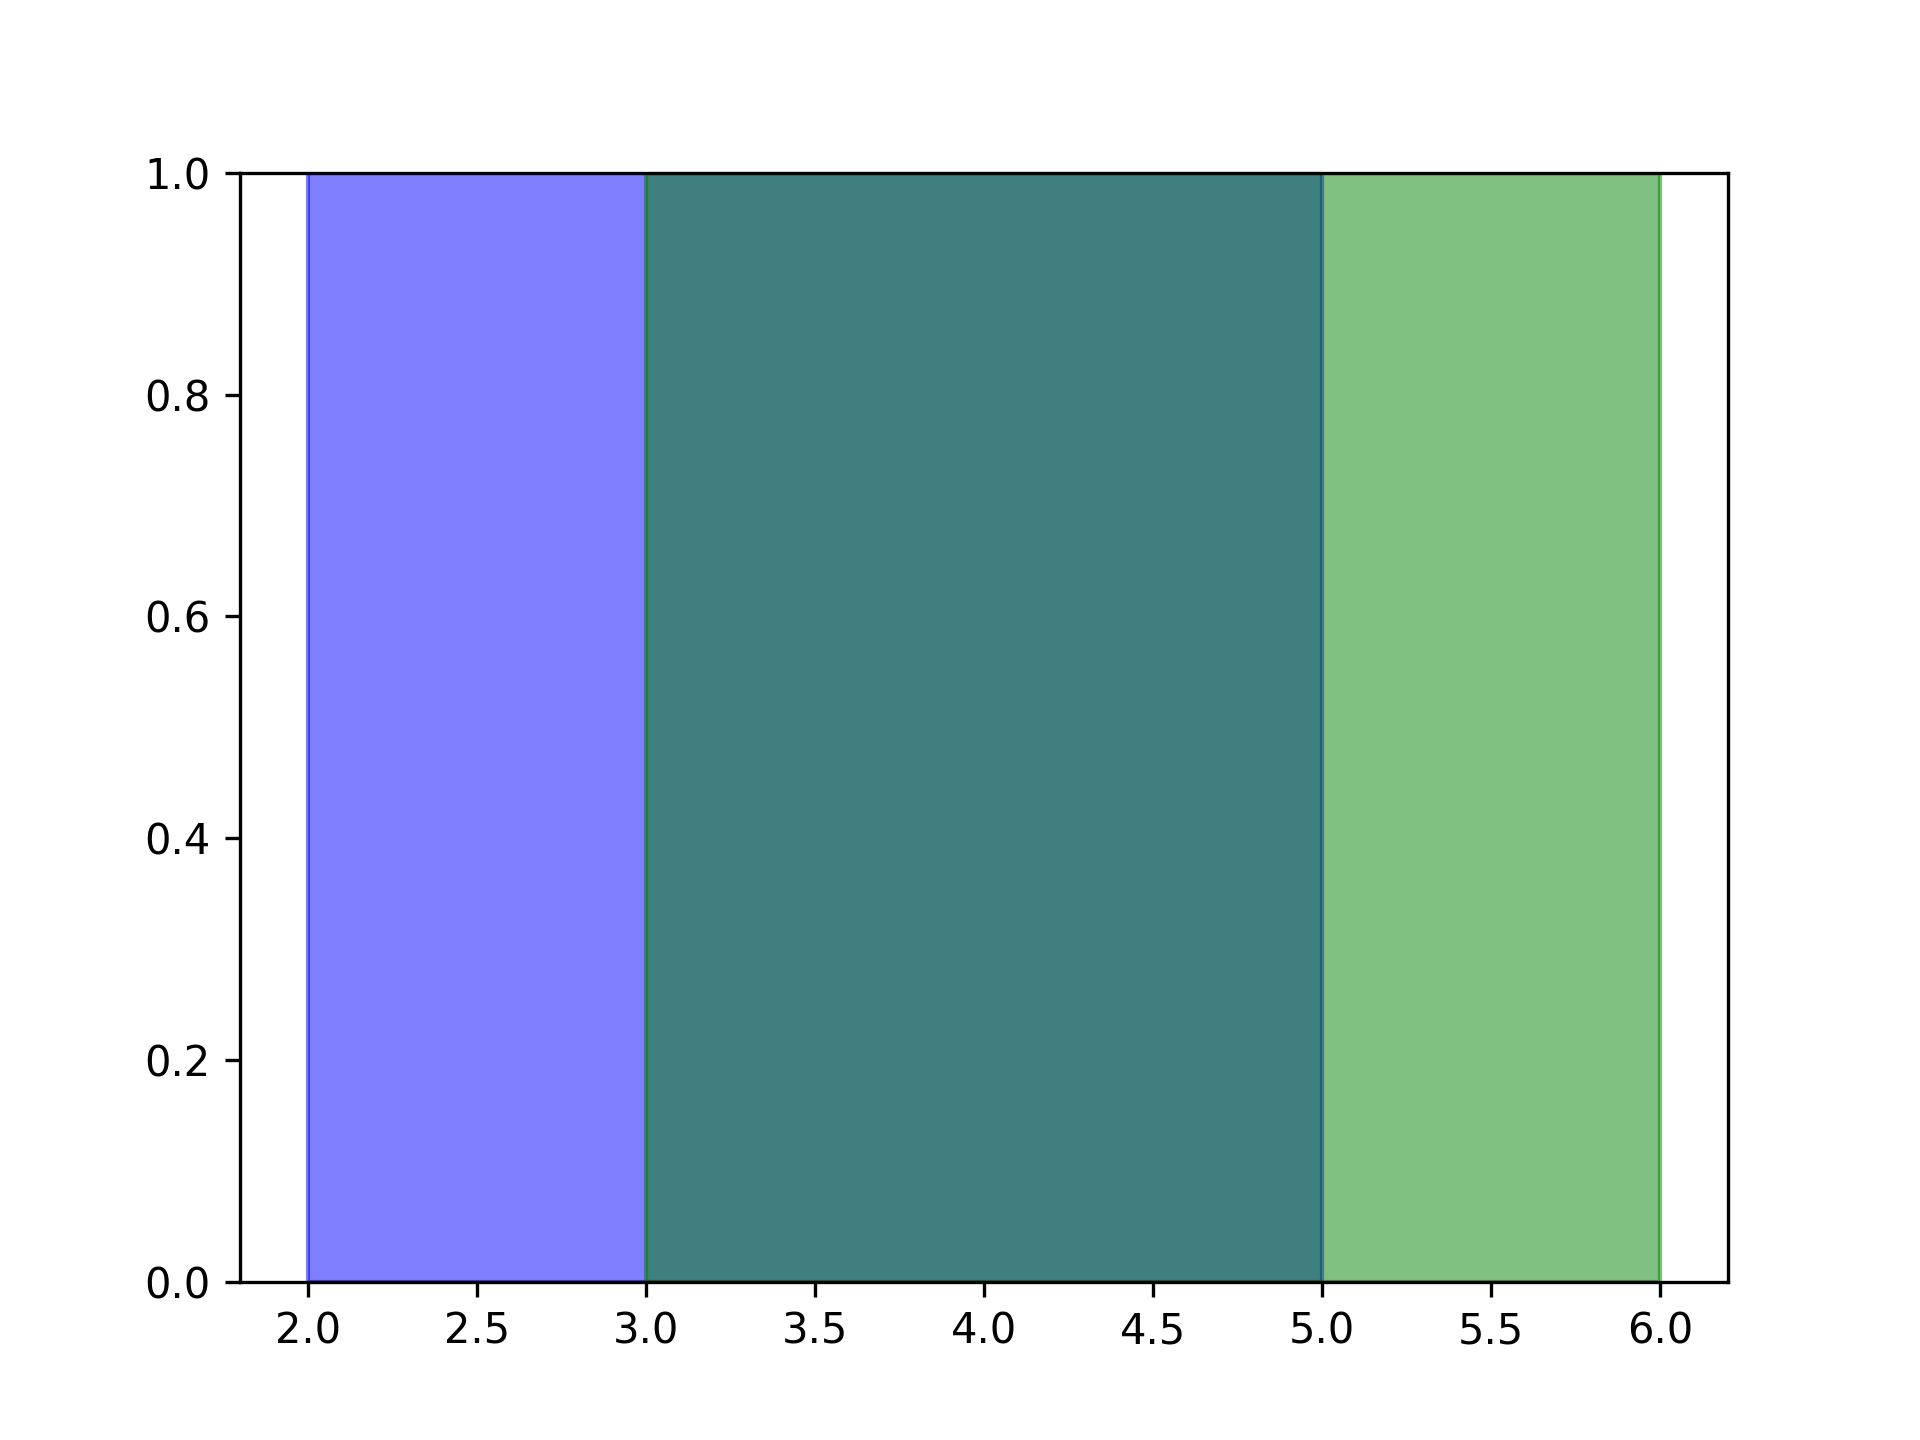
\includegraphics[width=0.65\textwidth]{coloring_region.png}
		\caption{Colored region of  A + B }
		\label{fig-1}
	\end{figure} 
\end{frame}


\section{Codes}
\begin{frame}{CODES}
    \begin{block}{Python}
         Download python code from - \href{https://github.com/Donal-08/Assignment-7/blob/main/code/line.py}{Python}
    \end{block}

 \begin{block}{Beamer}
         Download Beamer code from - \href{https://github.com/Donal-08/Assignment-7/blob/main/beamer.tex}{Beamer}
    \end{block}
\end{frame} 

\end{document}
